\begin{figure*}[t!]
    \centering
    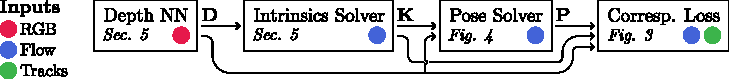
\includegraphics[width=\linewidth,]{figures/flowchart/fig_flowchart_pdf.pdf}
    \caption{\textbf{A FlowMap Forward Pass.}
    Given RGB frames (red), optical flow (blue) and point tracks (green), FlowMap computes dense depth $\depth$, camera poses $\pose$, and intrinsics $\ints$ in each forward pass. 
    We obtain depth via a CNN (\cref{sec:reparams}) and implement differentiable, feed-forward solvers for intrinsics and poses (\cref{sec:reparams}, Fig.\ref{fig:procrustes}).
    Colored dots indicate which block receives which inputs.
    FlowMap's only free parameters are the weights of a depth NN and a small correspondence confidence MLP.
    These parameters are optimized for each video separately by minimizing a camera-induced flow loss (Fig.~\ref{fig:loss}) via gradient descent, though fully feed-forward operation is possible.
    }
    \label{fig:flowchart}
    \vspace{-10pt}
\end{figure*}
